\subsection{Flyweight}
\label{flyweight}

\textbf{Scopo}: Strutturale \\
\textbf{Raggio d'azione}: Oggetti

\paragraph{Definizione} Il pattern Flyweight permette di utilizzare la condivisione per supportare in modo efficiente un gran numero di oggetti a granularità fine.

\begin{figure}[H]
    \centering
    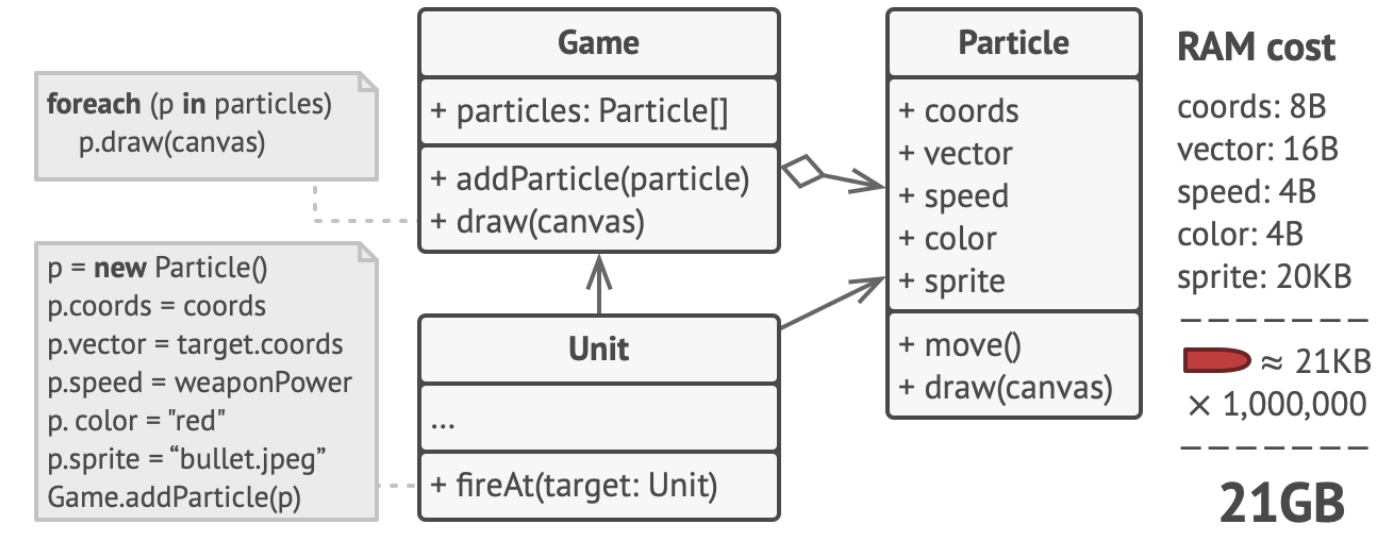
\includegraphics[width=1\linewidth]{assets/pattern/flyweight/flyweight-problema.png}
    \caption{Problema del particle system}
\end{figure}

\paragraph{Problema} Si consideri ad esempio un semplice videogioco in cui si è scelto di implementare un sistema particellare realistico e renderlo una caratteristica distintiva. Grandi quantità di proiettili, missili e schegge di esplosioni dovrebbero volare su tutta la mappa di gioco. Ogni particella è rappresentata da un oggetto separato contenente molti dati. Durante l’esecuzione, ad un certo punto, non c'è più spazio a sufficienza nella RAM per le particelle appena create, quindi il programma va in crash.

\begin{figure}[H]
    \centering
    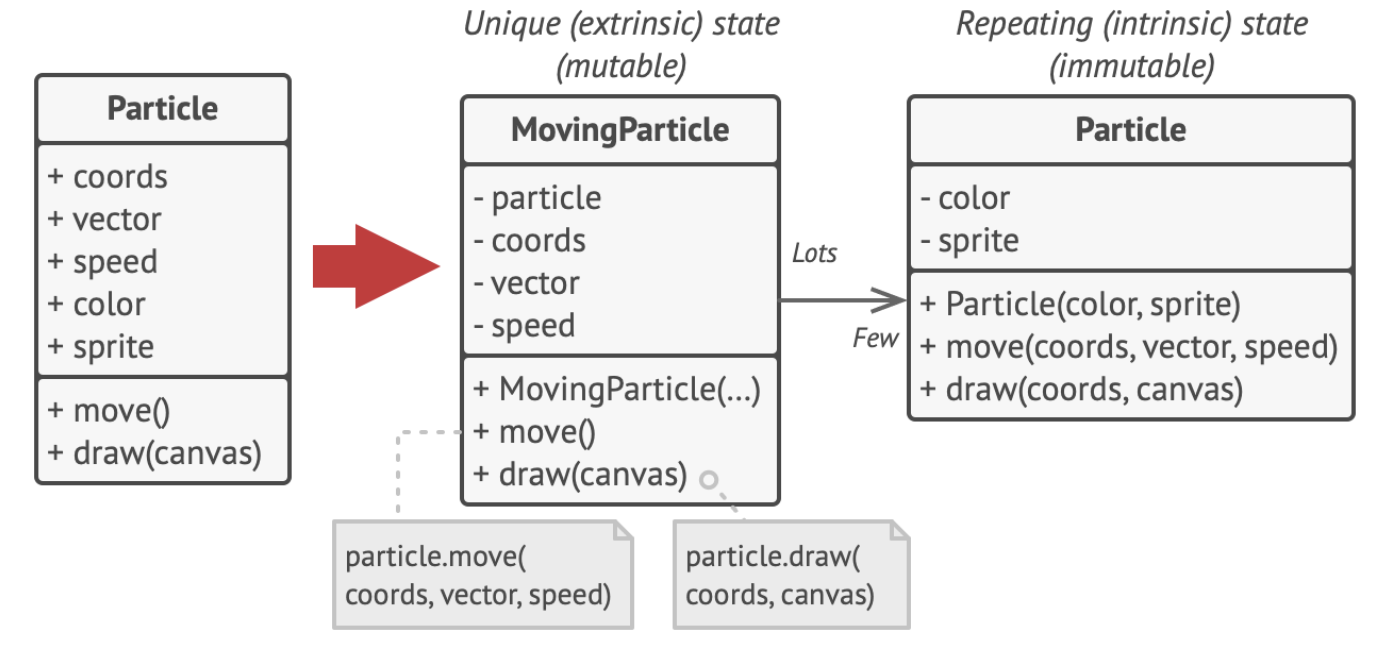
\includegraphics[width=1\linewidth]{assets/pattern/flyweight/flyweight-soluzione.png}
    \caption{Soluzione tramite pattern Flyweight}
\end{figure}

\paragraph{Soluzione} Il pattern Flyweight descrive come condividere oggetti in modo da consentire il loro uso a granularità fine senza avere costi proibitivi. Si costruisce un oggetto condiviso che può essere usato simultaneamente in più contesti. Data la loro natura c'è bisogno di distinguere tra stato interno (o intrinseco, informazioni indipendenti dal contesto) e stato esterno (o estrinseco, informazioni dipendenti dal contesto). Lo stato esterno viene passato dal client.

\begin{minipage}{0.5\linewidth}
    \paragraph{Esempio} Nell’esempio i campi color e sprite consumano molta più memoria rispetto agli altri. Inoltre essi memorizzano informazioni pressoché identiche tra le particelle. Ad esempio tutti i proiettili avranno lo stesso colore e lo stesso sprite. Gli altri campi, quali le coordinate, il vettore direzione e la velocità hanno valori distinti per ogni particella e inoltre cambiano con il tempo. Colore e sprite corrispondono allo stato intrinseco mentre gli altri campi allo stato estrinseco. La classe Particle modella lo stato intrinseco (immutabile), la classe MovingParticle quello estrinseco. Solo tre oggetti diversi saranno sufficienti a rappresentare lo stato esterno di tutte le particelle del gioco: uno per i proiettili, uno per il missili e uno per le schegge. Nell’esempio lo stato intrinseco è memorizzato nell’array particle della classe Game mentre quello estrinseco nell’array mps. Una soluzione più elegante consiste nell’introdurre una classe di contesto che memorizza lo stato estrinseco e un riferimento all’oggetto flyweight che corrisponde a quello intrinseco.
\end{minipage}
\hfill
\begin{minipage}{0.5\linewidth}
    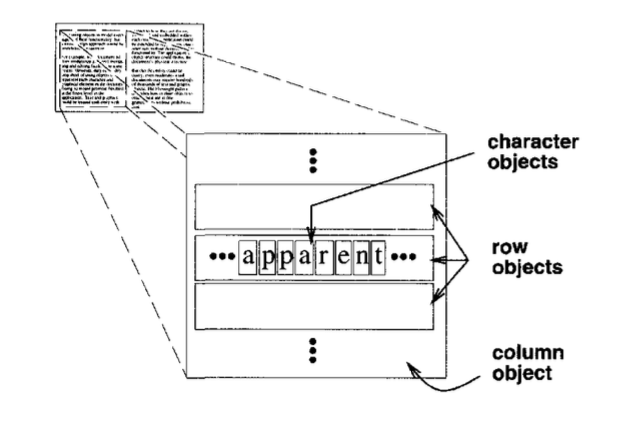
\includegraphics[width=1\linewidth]{assets/pattern/flyweight/flyweight-esempio.png}
\end{minipage}

\begin{figure}[H]
    \centering
    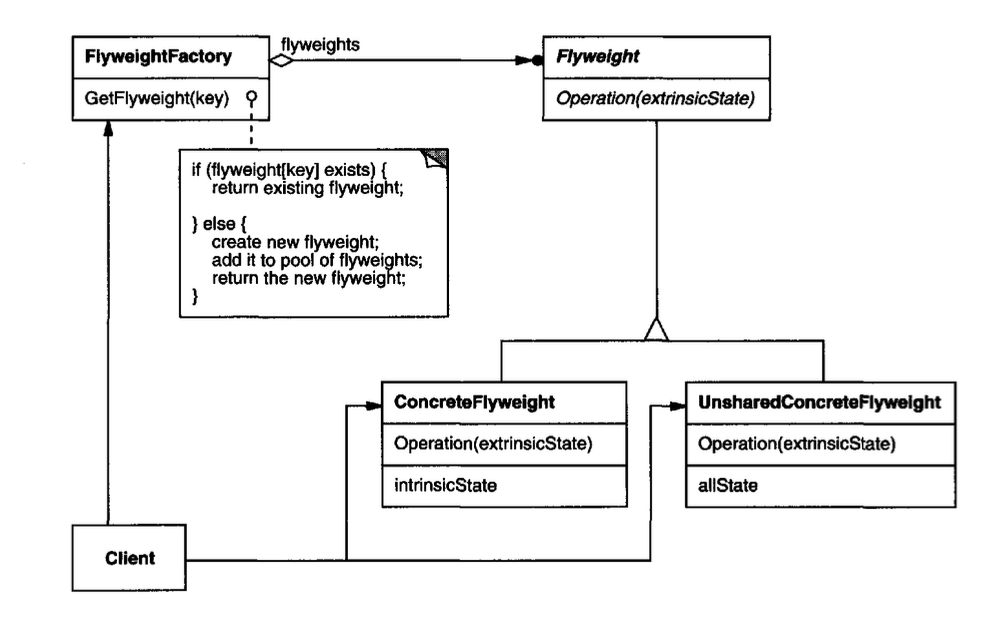
\includegraphics[width=1\linewidth]{assets/pattern/flyweight/flyweight-struttura.png}
    \caption{Class Diagram del pattern Flyweight}
\end{figure}

\paragraph{Struttura e Conseguenze} Il pattern è composto da:
\begin{itemize}
    \item \textbf{Flyweight}: dichiara un’interfaccia attraverso la quale gli oggetti flyweight possono ricevere lo stato esterno e agire di conseguenza.
    \item \textbf{FlyweightFactory}: crea e gestisce gli oggetti flyweight. Si assicura che i flyweight siano condivisi in modo appropriato. Quando un client richiede un flyweight, l’oggetto FlyweightFactory restituisce un’istanza esistente, oppure, se non esiste alcuna istanza, prima la crea e poi la restituisce.
    \item \textbf{Context}: contiene lo stato estrinseco, unico tra tutti gli oggetti originali. Quando un oggetto context è accoppiato con uno degli oggetti flyweight, rappresenta l’intero stato di un oggetto originale.
    \item \textbf{Client}: calcola oppure memorizza lo stato estrinseco dei flyweight. Dal punto di vista del client, un flyweight è un oggetto template che può essere configurato a tempo di esecuzione fornendogli dati contestuali come parametri dei suoi metodi.
\end{itemize}

\newpage